\chapter{Modelagem geológica implícita com funções distância assinaladas} \label{metodologia}

O método é baseado na interpolação de uma função implícita calculada para cada amostra e posterior definição de uma superfície de iso valores da função interpolada. A cada amostra é atribuída a distância euclideana anisotrópica entre ela mesma e a amostra mais próxima que pertence a um outro domínio geológico. O sinal da distância calculada revela se a amostra se encontra no interior (sinal negativo) ou exterior (sinal positivo) do domínio a ser modelado. A interpolação dessas medidas de distância permite a construção de um modelo binário de domínio geológico aplicando uma regra de corte (valor zero) na função implícita interpolada \cite{silvaanddeutschccgmodeling}. 

Ao contrário dos métodos visitados nas \autoref{sec_leapfrog} e \autoref{sec_campos}, que permitiam a modelagem de um domínio por vez, esse método permite modelar múltiplos domínios simultaneamente. Sendo assim, a categoria correspondente a menor distância estimada deve ser retida.

\section{Metodologia}\label{metodologia}

\subsection{Caso binário}\label{binario}

Primeiramente, o conjunto de dados ${z(u_\alpha),\alpha=1,...,n}$ é codificado em indicadores binários de acordo com a \autoref{eq_ind}, especificando se a amostra pertence ou não ao domínio. 

\begin{equation}
	i(u_\alpha)=\begin{cases}
	1,\:\textrm{se}\:z(u_\alpha)\:\textrm{se pertence ao domínio}\\
	0,\:\textrm{se}\:z(u_\alpha)\:\textrm{caso contrário}\end{cases}
    \label{eq_ind}
\end{equation}

\citeonline{maureira} apresentou um exemplo simples em duas dimensões para ilustrar o método. Na \autoref{indicadores} os pontos amostrais foram codificados em indicadores.

\begin{figure}[!ht]
	\caption{\label{indicadores}Transformação do banco de dados categóricos em indicadores binários.}
	\begin{center}
		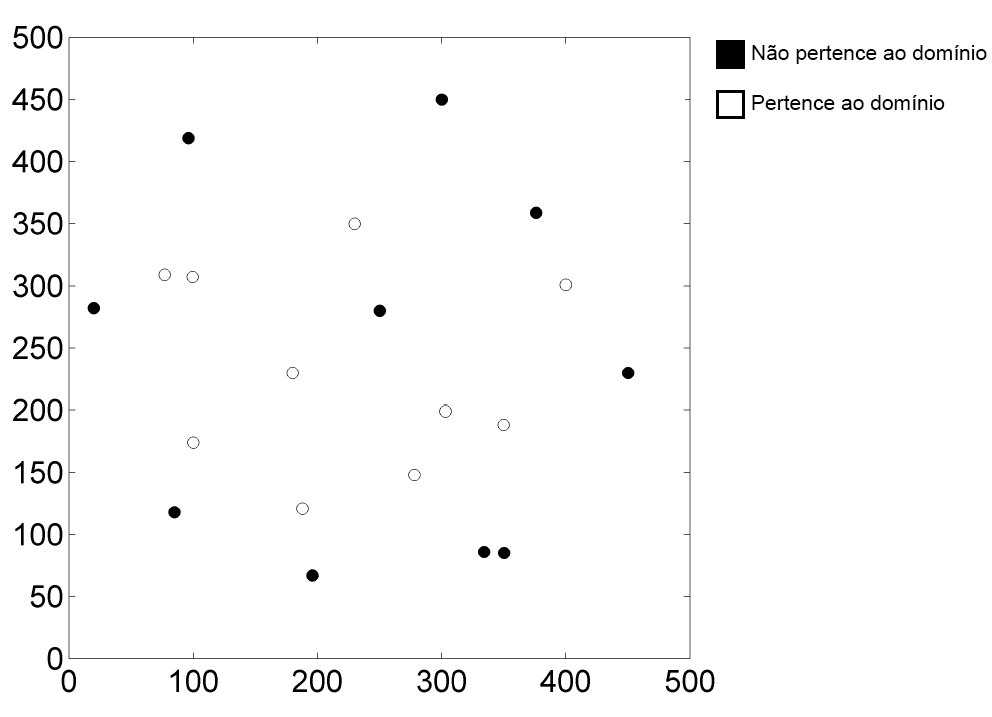
\includegraphics[width=0.5\textwidth]{modelagem_geologica/indicadores}
	\end{center}
	\legend{Fonte: Modificado de \citeonline{maureira}}
\end{figure}

Então, as distâncias assinaladas são calculadas para cada amostra de acordo com a \autoref{eq_sg}. Se a amostra pertence ao domínio modelado a distância é negativa, caso contrário positiva.

\begin{equation}
	d(u_\alpha)=\begin{cases}
	-\parallel u_\alpha-u_\beta\parallel,\:\textrm{se}\:i(u_\alpha)=1\\
	+\parallel u_\alpha-u_\beta\parallel,\:\textrm{se}\:i(u_\alpha)=0\end{cases}
    \label{eq_sg}
\end{equation}

O local $u_\beta$ corresponde à amostra mais próxima que pertença a um domínio diferente de $u_\alpha$. A regra euclideana é usada no cálculo.

A \autoref{distancias} mostra as distâncias assinaladas calculadas para cada ponto amostral.

\begin{figure}[!ht]
	\caption{\label{distancias}Função distância assinalada calculada para cada ponto amostral.}
	\begin{center}
		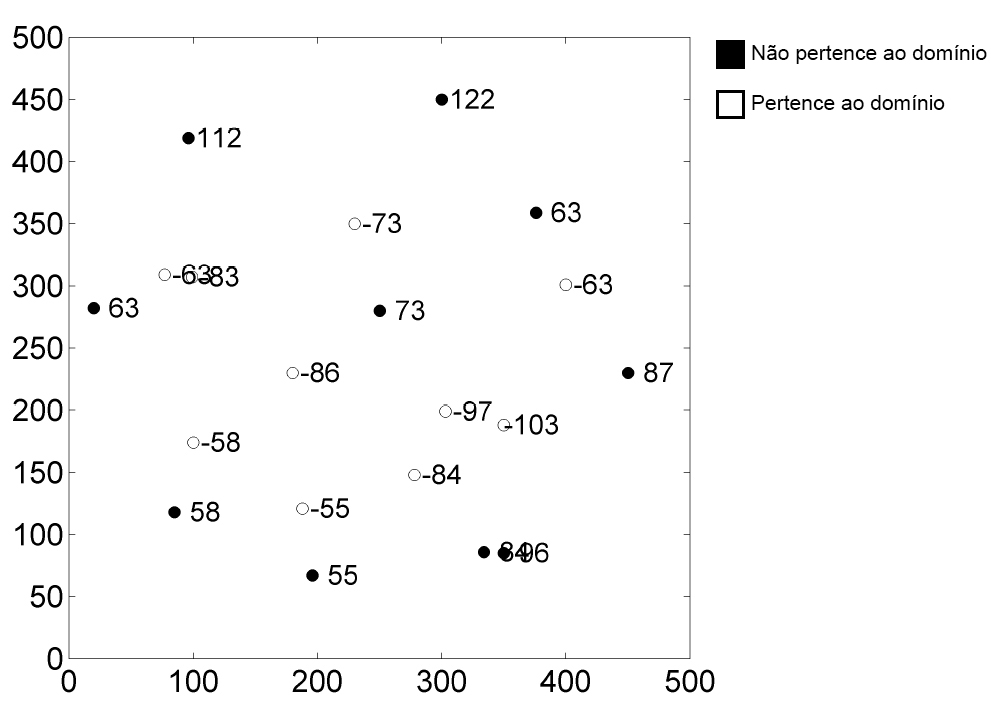
\includegraphics[width=0.5\textwidth]{modelagem_geologica/SG}
	\end{center}
	\legend{Fonte: Modificado de \citeonline{maureira}}
\end{figure}

Nos casos em que há o conhecimento de que o corpo geológico se estende mais em uma direção do que nas outras (como os corpos tabulares, por exemplo) as distâncias calculadas podem ser anisotrópicas. Assim sendo, as coordenadas originais $x$, $y$ e $z$ dos dados devem ser rotacionadas e/ou contraídas/dilatadas, a partir da transformação da \autoref{eq_rot_matrix}. Então, as distâncias euclideanas (\autoref{eq_sg}) são calculadas normalmente para as novas coordenadas $x''$, $y''$, $z''$.

\begin{equation}
\begin{gathered}
\begin{bmatrix} x'' \\ y'' \\ z'' \end{bmatrix} = \begin{bmatrix} \frac{1}{a_{max}} & 0 & 0 \\ 0 & \frac{1}{a_{min}} & 0 \\ 0 & 0 & \frac{1}{a_{vert}} \end{bmatrix} \\ \begin{bmatrix}\cos\alpha\cos\phi-\sin\alpha\sin\beta\sin\phi & -\sin\alpha\cos\phi-\cos\alpha\sin\beta\sin\phi & \cos\beta\sin\phi \\ \sin\alpha\cos\beta & \cos\alpha\cos\beta & \sin\beta \\ -\cos\alpha\sin\phi-\sin\alpha\sin\beta\cos\phi & \sin\alpha\sin\phi-\cos\alpha\sin\beta\cos\phi & \cos\beta\cos\phi \end{bmatrix} \begin{bmatrix} x \\ y \\ z \end{bmatrix}
\end{gathered}
	\label{eq_rot_matrix}
\end{equation}

Onde $a_{max}$, $a_{min}$ e $a_{vert}$ são as dimensões dos eixos máximo, médio e mínimo de anisotropia, e $\alpha$, $\beta$ e $\phi$, os ângulos de azimute, mergulho e \textit{rake}, respectivamente.   

A construção da função implícita em cada ponto amostral é a mesma para o método visitado na \autoref{sec_leapfrog}.

A função distância calculada para cada amostra é então interpolada para todos os pontos de interesse, a partir da \autoref{eq_OK}. Qualquer técnica de interpolação pode ser utilizada. Inverso da distância e krigagem produzem limites realísticos para os domínios. Porém, a krigagem permite levar em consideração a anisotropia e continuidade espacial das distâncias calculadas \cite{silvaanddeutschccgmodeling}.

\citeonline{silvaanddeutschccgmodeling,deutschcoal,maureira} recomendam que a krigagem global \cite{neufeld}, um interpolador suave que retém todas as amostras nas estimativas (não há estratégia de busca), seja utilizada. Desse modo, evita-se o surgimento de artefatos nos mapas gerados. Todavia, reter todas as amostras na interpolação pode aumentar consideravelmente o tempo de execução do algoritmo. Testes realizados no \autoref{estudo_de_caso} mostraram que o uso da krigagem ordinária com uma vizinhança de busca e número de amostras retidas suficientemente grandes, produzem um resultado muito semelhante à krigagem global.

\begin{equation}
	d^*(u)=\sum\limits_{\alpha=1}^n \lambda_\alpha^{OK}(u)d(u_\alpha)
    \label{eq_OK}
\end{equation}

Onde $d^*(u)$ é a distância estimada para cada local não amostrado $u$, $\lambda_\alpha^{OK}(u)$ os pesos de krigagem ordinária e $d(u_\alpha)$ o valor da função distância assinalada calculado para cada amostra.

A \autoref{interpolated} mostra a função distância interpolada por krigagem ordinária em todos os pontos de interesse.

\begin{figure}[!ht]
	\caption{\label{interpolated}Função distância interpolada para todos os locais de interesse.}
	\begin{center}
		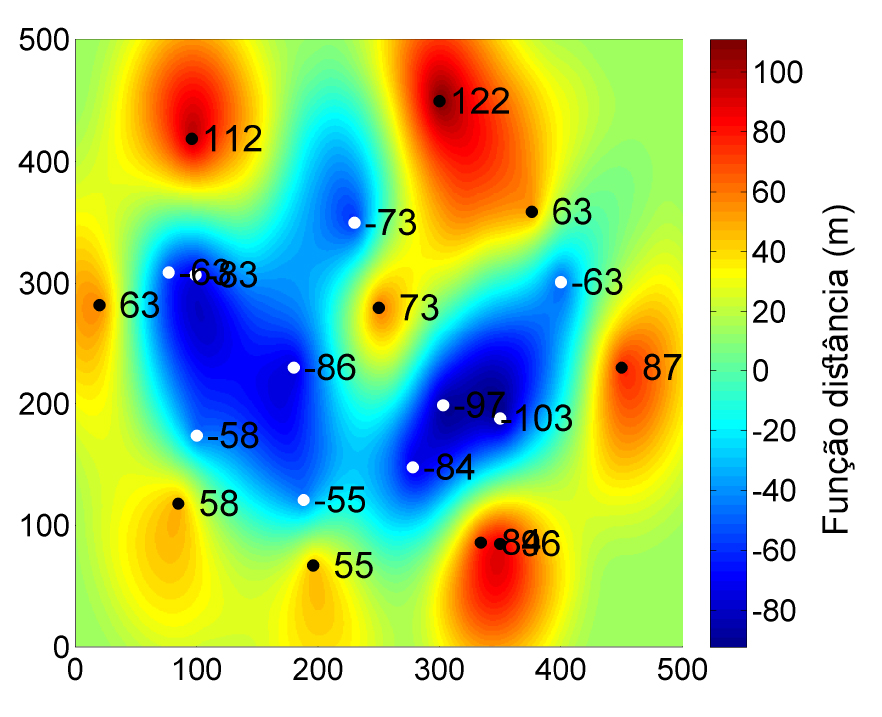
\includegraphics[width=0.5\textwidth]{modelagem_geologica/interpolated}
	\end{center}
	\legend{Fonte: Modificado de \citeonline{maureira}}
\end{figure}

Por fim, cada local de interesse é classificado com base no sinal da função distância interpolada, de acordo com a \autoref{classifier}. Blocos em que a função tem valor negativo, são classificados como pertencentes ao domínio. Blocos em que a função tem valor positivo, classificados como não pertencentes ao domínio.

Como as funções distância são negativas no interior do domínio e positivas no exterior, um bom palpite inicial para a interface que separa os domínios no espaço, seria a linha (em duas dimensões) ou superfície (em três dimensões) que corresponda ao valor zero da função distância assinalada \cite{wildedeutschcalibrate}. 

\begin{equation}
	i^*(u)=\begin{cases}
	1,\:\textrm{se}\:d^*(u)\leq0\\
	0,\:\textrm{caso contrário}\end{cases}
    \label{classifier}
\end{equation}

A \autoref{model} mostra o modelo geológico criado para o domínio a partir do sinal da função distância interpolada (\autoref{interpolated}).

\begin{figure}[!ht]
	\caption{\label{model}Modelo geológico criado a partir do sinal da função distância interpolada.}
	\begin{center}
		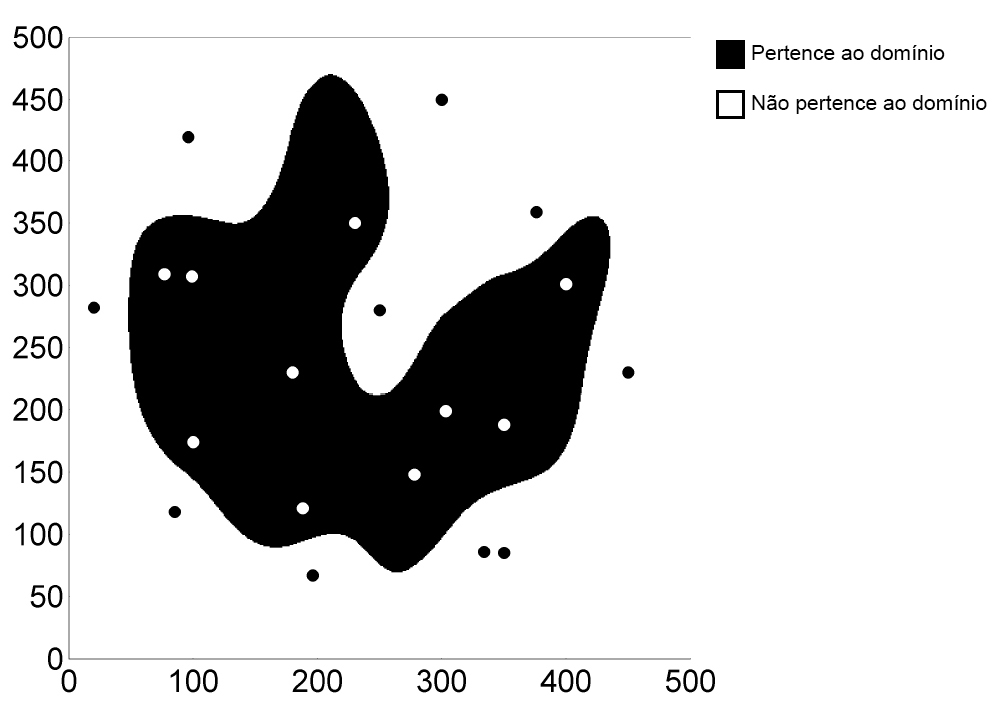
\includegraphics[width=0.5\textwidth]{modelagem_geologica/modelo}
	\end{center}
	\legend{Fonte: Modificado de \citeonline{maureira}}
\end{figure}

\subsection{Aplicação da metodologia para múltiplos domínios geológicos}

A metodologia apresentada na \autoref{binario} é adequada apenas para casos binários, na presença de múltiplas categorias \citeonline{silvaanddeutschccgmodeling} propuseram, também, uma metodologia. O objetivo é modelar os diversos domínios geológicos simultaneamente de forma similar ao caso binário.

Se existirem $K$ múltiplos domínios no depósito mineral, para cada ponto amostral ${z(u_\alpha),\alpha=1,...,n}$, um vetor de indicadores de $K$ elementos é codificado de acordo com a \autoref{eq_mult_ind}.

\begin{equation}
	i_k(u_\alpha)=\begin{cases}
	1,\:\textrm{se}\:z(u_\alpha)=k\\
    0,\:\textrm{se}\:z(u_\alpha)\:\textrm{caso contrário}\end{cases} k=1,...,K
    \label{eq_mult_ind}
\end{equation}

As amostras são codificadas $K$ vezes, uma vez para cada domínio.

Da mesma forma que na \autoref{eq_sg}, a função distância é calculada, individualmente para cada elemento $k$ do vetor, de acordo com a \autoref{eq_mult_sg}.

\begin{equation}
	d_k(u_\alpha)=\begin{cases}
	-\parallel u_\alpha-u_\beta\parallel,\:\textrm{se}\:i_k(u_\alpha)=1\\
	+\parallel u_\alpha-u_\beta\parallel,\:\textrm{se}\:i_k(u_\alpha)=0\end{cases} k=1,...,K
    \label{eq_mult_sg}
\end{equation}

Diferentes anisotropias podem ser incorporadas para cada categoria, a correlação entre as distâncias calculadas não é considerada.

As distâncias calculadas são então interpoladas, individualmente, para cada categoria, de acordo com a \autoref{eq_mult_ok}.

\begin{equation}
	d_k^*(u)=\sum\limits_{\alpha=1}^n \lambda_\alpha^{OK}(u)d_k(u_\alpha)\quad k=1,...,K
    \label{eq_mult_ok}
\end{equation}

Quando os múltiplos variogramas são similares, um único modelo pode se considerado.

Por fim, cada bloco é  classificado pela \autoref{eq_mult_rt}

\begin{equation}
	i^*(u)=k'\;\text{de modo que}\;d_{k'}^*=min\{d_k^*(u)\}_{k=1}^K
    \label{eq_mult_rt}
\end{equation}

As distâncias estimadas fornecem uma medida de proximidade ao domínio oposto mais próximo. Sendo assim, a mínima distância assinalada estimada é tida como o domínio mais provável de ser encontrado numa região não amostrada. A \autoref{eq_mult_rt} sumariza essa ideia \cite{maureira}. A categoria associada com a menor distância estimada é carimbada em cada bloco.

A \autoref{mult_cat} mostra um exemplo de um modelo geológico criado a partir da mínima distância assinalada estimada. A esquerda, a figura mostra a projeção das distâncias assinaladas para cada uma das quatro categorias, e à direita a classificação final.

\begin{figure}[!ht]
	\caption{\label{mult_cat}Função distância interpolada para todos os locais de interesse.}
	\begin{center}
		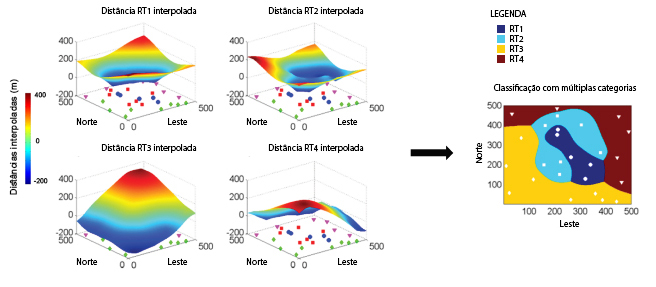
\includegraphics[width=0.8\textwidth]{modelagem_geologica/mult_cat_legenda}
	\end{center}
	\legend{Fonte: Modificado de \citeonline{silvageostatlessons}}
\end{figure}

\section{Uma medida heurística de incerteza (\textit{softmax transformation})}\label{softmax_chap}

A metodologia proposta por \citeonline{silvaanddeutschccgmodeling} não caracteriza a incerteza associada ao modelo geológico. \citeonline{maureira} apresentou uma forma heurística para determinação da incerteza, essa metodologia não é baseada em múltiplas realizações de uma função aleatória, é um pós processamento derivado de uma transformação.

Várias formas de determinar a incerteza para métodos determinísticos de modelagem geológica implícita foram desenvolvidos. \citeonline{mclennan2006implicit} propuseram uma metodologia para quantificar a incerteza de volumes geológicos criados a partir de funções volume (muito similares às funções distância assinaladas) a partir da técnica de \textit{bootstrap sampling}. \citeonline{munroe2012methodology} propôs calibrar uma banda de incerteza ao longo dos contatos entre os domínios, uma ideia similar foi implementada por \citeonline{wildedeutschcalibrate}, onde a incerteza é considerada diretamente na krigagem, adicionando uma constante às estimativas.

As distâncias estimadas em cada bloco para cada categoria carregam consigo informação adicional. Como já discutido, as distâncias estimadas fornecem uma medida de proximidade à interface mais próxima. Então, as distâncias podem ser estandardizadas entre zero e um, fornecendo uma medida de incerteza \cite{maureira}.

\subsubsection{Transformação das distâncias}

\textit{Softmax transformation} é uma técnica amplamente usada em métodos de classificação para múltiplas classes \cite{mccullagh}. A ideia é transformar as distâncias estimadas em probabilidades a partir da \autoref{eq_softmax}. Os valores transformados encontram-se entre zero e um e  sua soma deve ser igual a um, para cada bloco estimado.

\begin{equation}
	P(i(u)=k)=\frac{e^\frac{-d^*_k(u)}{\gamma}}{\sum_{k'=1}^{K}e^\frac{-d^*_k(u)}{\gamma}}
    \label{eq_softmax}
\end{equation}

$P(i(u)=k)$ representa a probabilidade de um local $u$ pertencer à categoria $k$, $d^*_k(u)$ é a distância estimada para a categoria $k$ e $\gamma$ é um parâmetro que regula a inter-relação entre as probabilidades das $K$ diferentes categorias. Quanto maior $\gamma$, maior as diferenças entre as probabilidades (maior a banda de incerteza), como pode ser observado na \autoref{softmax_gamma}.

\begin{figure}[!ht]
	\caption{\label{softmax_gamma}Mapas de probabilidades gerados com dois valores de gamma diferentes. À esquerda $\gamma=80$, à direita $\gamma=175$.}
	\begin{center}
		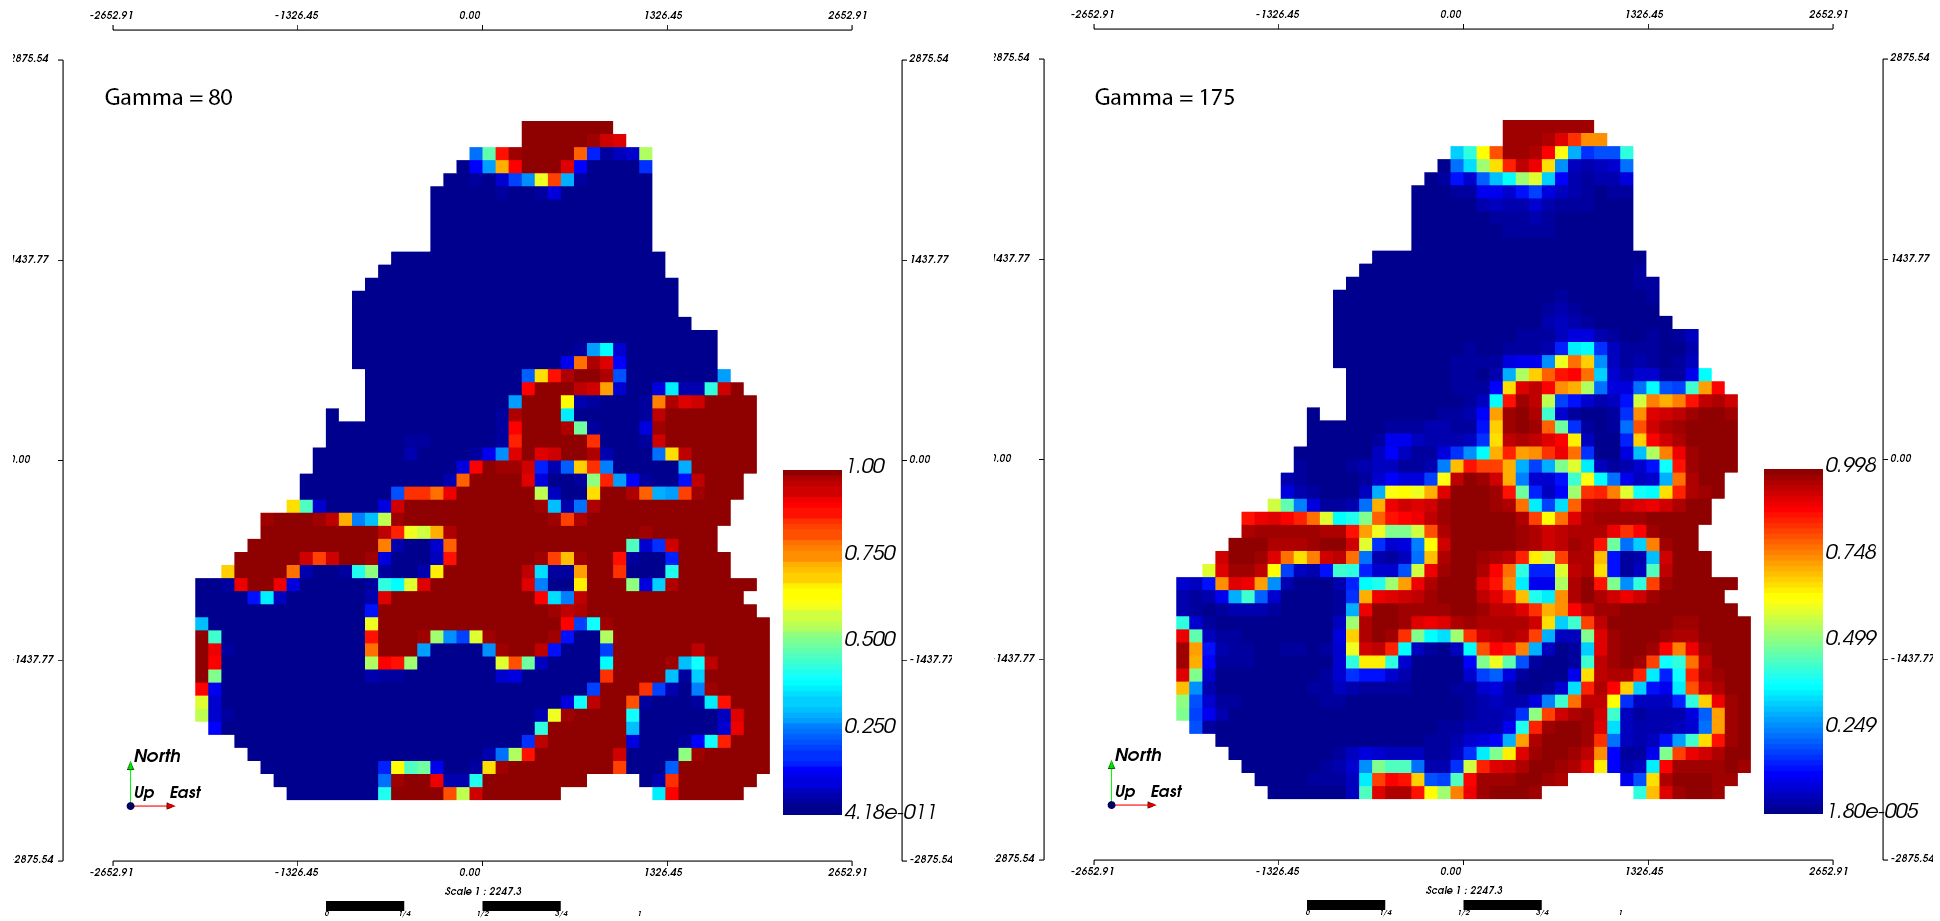
\includegraphics[width=0.6\textwidth]{modelagem_geologica/softmax_gama}
	\end{center}
	%\legend{Fonte: Modificado de \citeonline{maureira}}
\end{figure}

Para exemplificar a transformação, a \autoref{softmax_grafico}, mostra à esquerda as distâncias estimadas para cada uma de cinco categorias em um mesmo bloco em particular. À direita as distâncias transformadas pela \autoref{eq_softmax} em probabilidades daquele bloco pertencer a cada uma das cinco categorias. Observe que distâncias menores (mais negativas) geram probabilidades maiores, e vice-versa.  

\begin{figure}[!ht]
	\caption{\label{softmax_grafico}Distâncias estimadas e transformadas em probabilidades para um mesmo bloco.}
	\begin{center}
		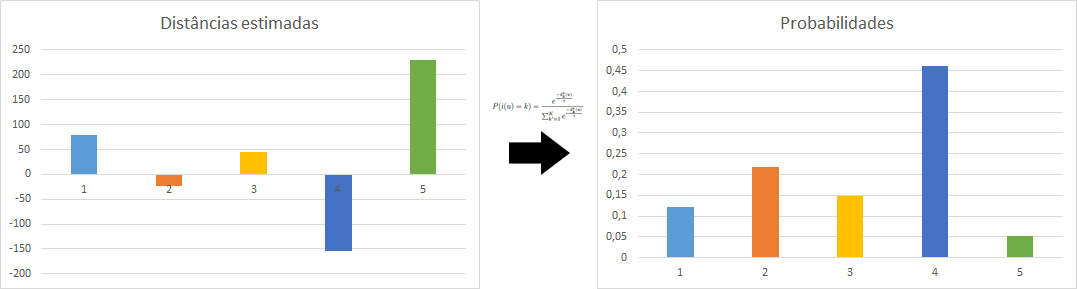
\includegraphics[width=0.7\textwidth]{modelagem_geologica/softmax_bars_final}
	\end{center}
	%\legend{Fonte: Modificado de \citeonline{silvageostatlessons}}
\end{figure}

\section{Correção das proporções globais dos domínios (\textit{servo system})}\label{servo_chap}

Uma das preocupações durante a modelagem geológica implícita de domínios geológicos é quanto à inserção de viés nos modelos. O viés pode ser proveniente da interação entre os parâmetros e o algoritmo, da variabilidade geológica ou da configuração da malha de amostragem.

Tipicamente, as campanhas de sondagem têm como foco áreas de altos teores. Como se espera obter lucro ainda nos primeiros anos de operação, mais informação das áreas mais ricas do depósito é fundamental. Essa prática é conhecida como amostragem preferencial e pode levar ao cálculo enviesado das proporções de cada domínio, caso não receba o tratamento devido. Existem diversas técnicas de desagrupamento disponíveis, dentre as mais utilizadas, o método dos polígonos e método das células \cite{maureira}.

\citeonline{maureira} propôs, como uma extensão do algoritmo, gerar modelos que correspondem às estatísticas representativas (desagrupadas) dos domínios do depósito. Essas proporções são calculadas a partir das probabilidades obtidas através da \textit{softmax tranformation}.

\subsection{\textit{Servo system}}

A correção com \textit{servo system} foi introduzida por \citeonline{strebelle2000sequential} e objetiva ajustar a probabilidade marginal ao longo do processo iterativo de simulação por MPS em cada nó.

A técnica possibilita reproduzir um conjunto de proporções pré-definido, as proporções observadas nos dados desagrupados, por exemplo. A ideia central do algoritmo é atualizar as probabilidades para cada domínio, em cada nó, baseado na diferença entre a proporção alvo e a proporção marginal corrente (proporção encontradas nos blocos visitados até então) (\autoref{eq_servo}), a intensidade da correção é proporcional à magnitude da diferença.

\begin{equation}
	P(i(u)=k)^\text{update}=P(i(u)=k)+\mu(p(k)-P_k^c(u))
	\label{eq_servo}
\end{equation}

$P(i(u)=k)^\text{update}$ é a probabilidade atualizada em cada bloco $u$, $P(i(u)=k)$ é a probabilidade para o bloco $u$ calculada a partir da \textit{softmax transformation}, $\mu$ é o parâmetro que controla a intensidade da correção, e vale $\mu=\frac{\lambda}{1-\lambda}$, quanto mais próximo de um $\lambda$ for, mais correção nas proporções. $p(k)$ e $P_k^c(u)$ são respectivamente, a proporção alvo e a proporção marginal corrente para a litologia $k$. O algoritmo deve visitar os blocos em um caminho aleatório para evitar o surgimento de artefatos nos modelos gerados.

Após as probabilidades de cada bloco pertencer a cada litologia serem atualizadas com a \autoref{eq_servo}, um novo modelo geológico deve ser gerado a partir da \autoref{eq_class_servo}.

\begin{equation}
	i^*(u)=\text{argmax}P(i(u)=k)^\text{updated}
    \label{eq_class_servo}
\end{equation}

Cada bloco é reclassificado, não mais pela menor distância estimada, mas pela maior probabilidade atualizada.

Muitas vezes, a escolha do parâmetro $\mu$ (muito alta), gera modelos com aparência granulada ou \textit{salt and pepper} (\autoref{servosystem_salt} à esquerda), que não fazem sentido físico. Uma fase de pós processamento para suavizar o modelo está embutida no algoritmo do \textit{servo system} (duas novas propriedades são criadas, uma não corrigida e uma corrigida). Cada nó do \textit{grid} é visitado seguindo um caminho aleatório, novamente para evitar o surgimento de artefatos nos modelos. Um cubo de dimensões $3x3x3$ blocos cúbicos é centrado no bloco visitado e a proporção de cada litologia é calculada, considerando apenas os blocos abrangidos pelo cubo. A litologia que apresenta a maior proporção é carimbada no bloco visitado, metodologia semelhante é utilizada em classificação de recursos minerais.

A \autoref{servosystem_salt} mostra um modelo gerado com um parâmetro $\lambda=0.99$ à esquerda e um modelo gerado com $\lambda=0$, ou seja, um modelo sem correção baseado na menor distância estimada.

\begin{figure}[!ht]
	\caption{\label{servosystem_salt}Modelos geológicos gerados, sem correção das proporções à direita e com correção, usando um fator $\lambda = 0,99$ à esquerda.}
	\begin{center}
		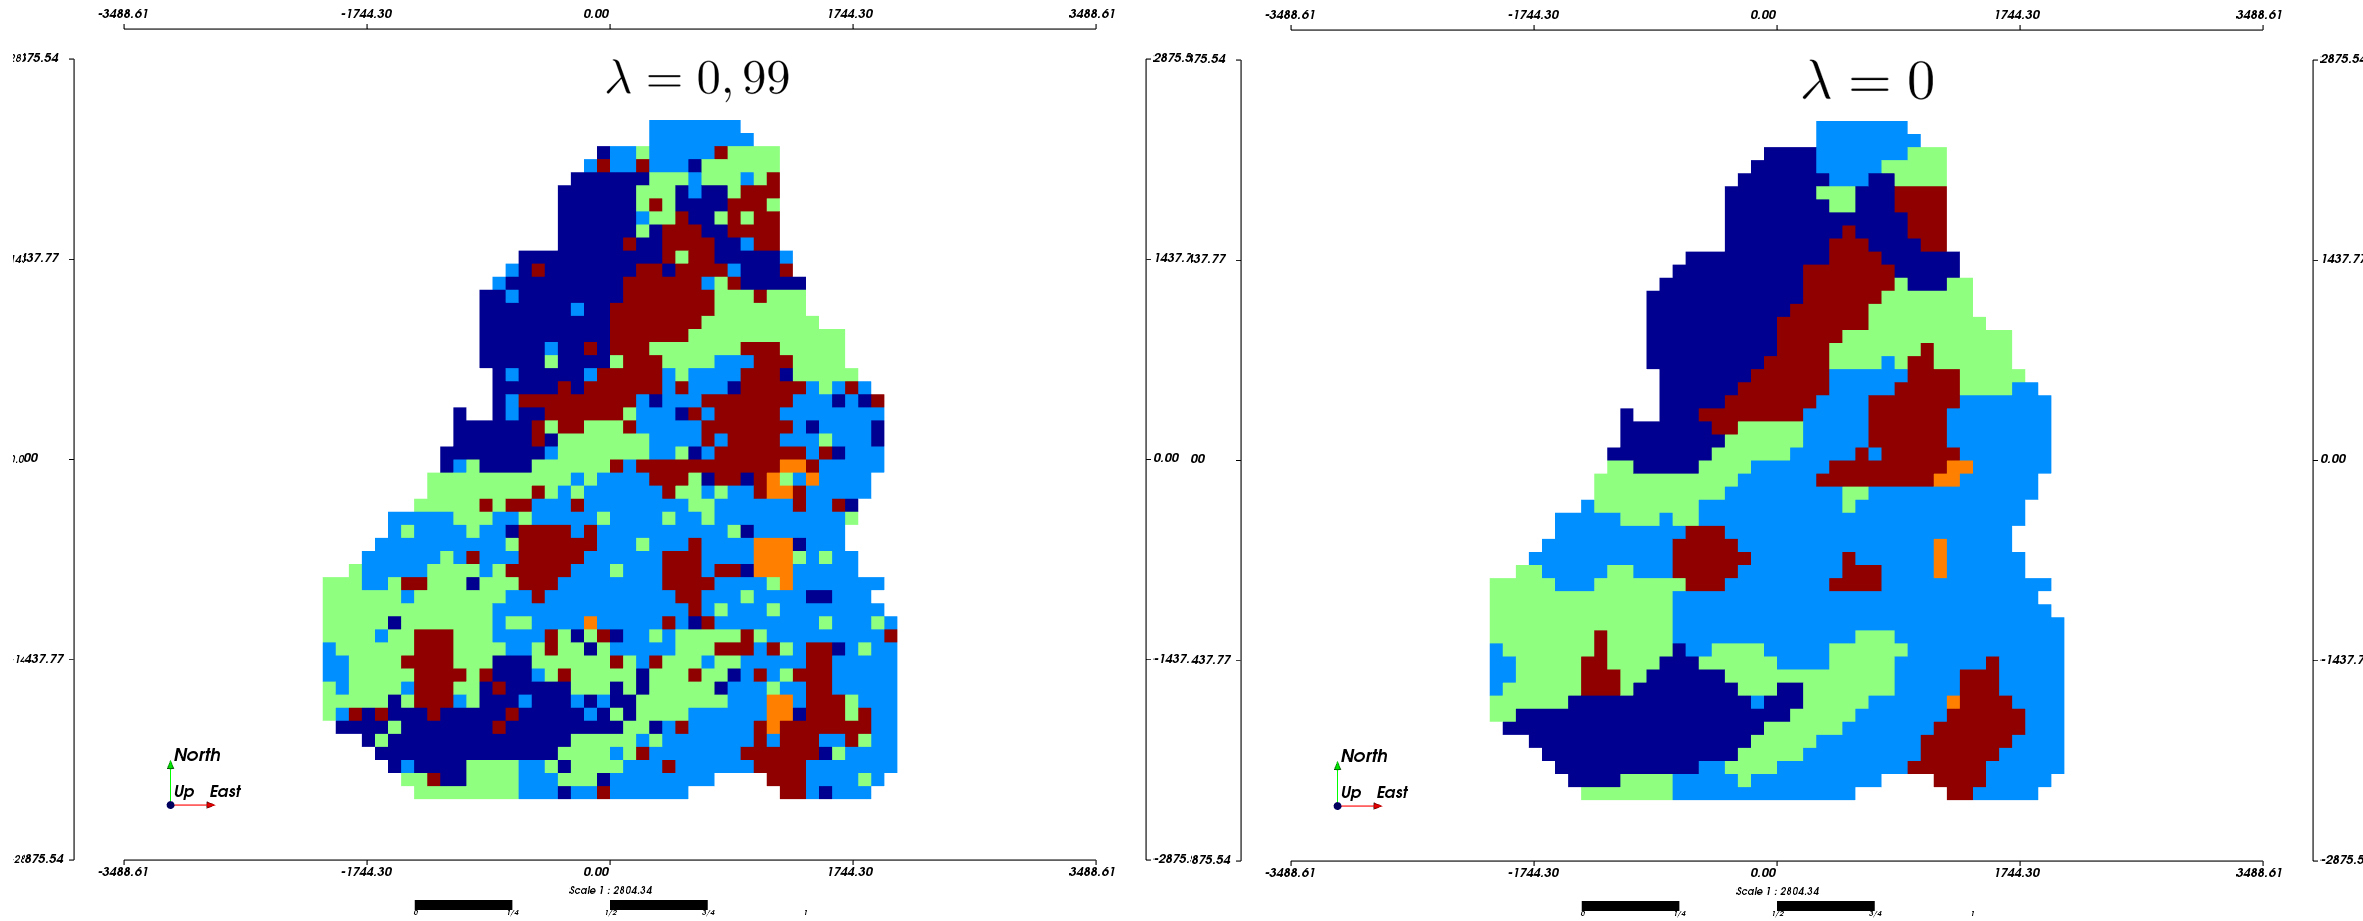
\includegraphics[width=0.6\textwidth]{modelagem_geologica/servosystem}
	\end{center}
	%\legend{Fonte: Modificado de \citeonline{maureira}}
\end{figure}

Alguns modelos podem apresentar efeito de borda, quando a influência de amostras localizadas nas bordas da malha de sondagem é extrapolada com exagero pelo algoritmo, criando estruturas inverossímeis. A aplicação do \textit{servo system} também controla a extensão desse tipo de estrutura, reduzindo o efeito de borda.

\section{O \textit{Plug-in}}

O método foi operacionalizado no \textit{software} geoestatístico de código aberto \textit{SGeMS}, com a criação de dois \textit{plug-ins} em linguagem \textit{python}. Os códigos podem ser encontrados no \autoref{apendicea} e \autoref{apendiceb}, bem como no repositório \textit{online} \url{https://github.com/LPM-UFRGS/dfmod}

No painel de algoritmos, há a opção \textit{DFMod} (\autoref{main_plugin}), que traz dois \textit{plugins}: \textit{signed distances} e \textit{interpolator}. O primeiro calcula o valor da função distância assinalada para cada amostra e para cada litologia. O segundo interpola a função distância, usando krigagem ordinária, para todo o \textit{grid}, além de apresentar opções de calcular a incerteza com \textit{softmax transformation} (\autoref{softmax_chap}) e corrigir as proporções com \textit{servo system} (\autoref{servo_chap}).

\begin{figure}[!ht]
	\caption{\label{main_plugin}Visão do painel de algoritmos do \textit{SGeMS} mostrando a opção \textit{DFMOD}.}
	\begin{center}
		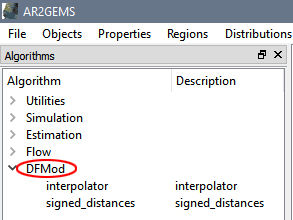
\includegraphics[width=0.5\textwidth]{modelagem_geologica/main}
	\end{center}
	%\legend{Fonte: Modificado de \citeonline{maureira}}
\end{figure}

\subsection{\textit{Signed distances}}\label{plugin_sg}

O \textit{plugin signed distances} (\autoref{sg_plugin}) calcula, para uma propriedade categórica, o valor da função distância anisotrópica (ou isotrópica), para cada amostra e cada litologia. O \textit{SGeMS} aceita apenas litologias codificadas em caracteres numéricos.   

\begin{figure}[H]
	\caption{\label{sg_plugin}Visão do \textit{plugin signed distances}.}
	\begin{center}
		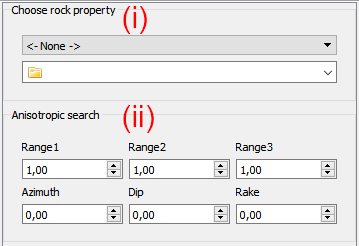
\includegraphics[width=0.5\textwidth]{modelagem_geologica/sg_plugin}
	\end{center}
	%\legend{Fonte: Modificado de \citeonline{maureira}}
\end{figure}

Em (i), usuário deve imputar a propriedade que informa a litologia (\textit{rock type}) de cada amostra. Em (ii), o usuário imputa os ângulos de rotação e razões de anisotropia, para o cálculo das distâncias anisotrópicas, o valor padrão calcula distâncias isotrópicas.

Como \textit{output}, o plugin gera uma propriedade \textit{signed distances RTX} para cada litologia, onde $X$ é o algarismo que representa aquela litologia.

O quadro Algoritmo 1 abaixo, mostra o funcionamento do algoritmo.

\begin{algorithm}[!ht]
\KwIn{Banco de dados categórico, ângulos de rotação e razões de anisotropia}
\KwOut{Propriedades \textit{signed distances RTX}}
Cria a matriz de rotação - dilatação/compressão\;
Transforma os dados originais $x,y,z$ em $x'',y'',z''$ com a matriz criada\;
Codifica as amostras, para cada domínio $k$, em $i_k(u_\alpha)$\; 
\For{litologias}{
	\For{amostras}{Calcula a distância entre cada amostra e todas as demais que pertencem a um domínio oposto\;
    Retém a distância mínima para cada amostra em uma lista\;
    Assinala de acordo com o indicador
}
Cria uma uma propriedade para cada litologia, referente a lista de menores distâncias criada em cada amostra (\textit{signed distances RTX})
}
\caption{Signed distances}
\end{algorithm}
 
\subsection{\textit{Interpolator}}\label{interpolator_sec}

O \textit{plugin interpolator} apresenta três abas: \textit{general, variogram} e \textit{options}. Na primeira aba (\autoref{interpolator_plugin}), o usuário deve imputar em (i) a propriedade categórica, nesse caso, para que os blocos que coincidem com amostras sejam carimbados com a respectiva litologia. Em (ii), o \textit{grid} no qual as distâncias serão interpoladas. Em (iii), o usuário deve imputar todas as distância \textit{signed distances RTX} calculadas com o \textit{plugin signed distances} (\autoref{plugin_sg}). Em (iv), a estratégia de busca da krigagem originária deve ser informada, número máximo e mínimo de dados condicionantes e elipsoide de busca.

\begin{figure}[H]
	\caption{\label{interpolator_plugin}Visão da aba \textit{general} do \textit{plugin interpolator}.}
	\begin{center}
		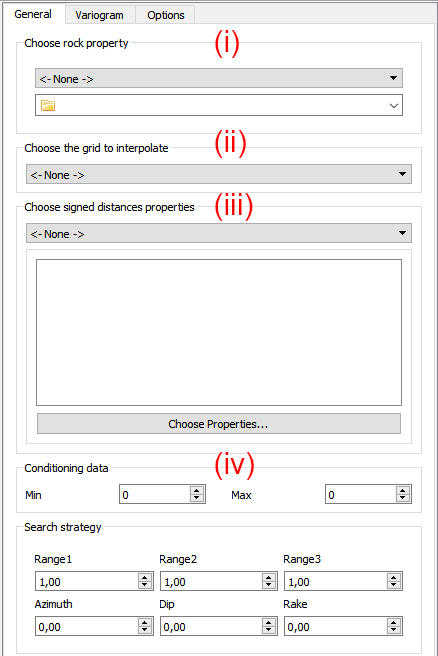
\includegraphics[width=0.5\textwidth]{modelagem_geologica/interpolator_plugin}
	\end{center}
	%\legend{Fonte: Modificado de \citeonline{maureira}}
\end{figure}

Na segunda aba (\autoref{variogram_plugin}), os modelos variográficos referentes a cada uma das propriedades \textit{signed distances RTX}, devem ser informados, na mesma ordem em que foram escolhidos na aba anterior (\autoref{interpolator_plugin} - (iii)). 

\begin{figure}[H]
	\caption{\label{variogram_plugin}Visão da aba \textit{variogram} do \textit{plugin interpolator}.}
	\begin{center}
		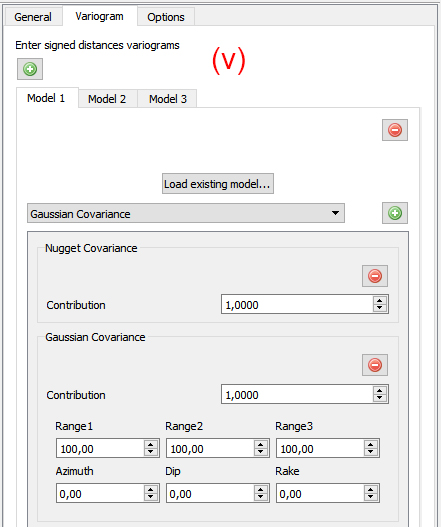
\includegraphics[width=0.5\textwidth]{modelagem_geologica/variogram_plugin}
	\end{center}
	%\legend{Fonte: Modificado de \citeonline{maureira}}
\end{figure}

Na terceira e última aba (\autoref{options_plugin}), o usuário escolhe se o modelo será pós processado. Em (vi), a opção \textit{softmax transformation} deve ser marcada, assim como o parâmetro $\gamma$ informado, em (vii), a opção \textit{servo system} deve ser marcada, o parâmetro $\lambda$ informado e a propriedade para a qual se deseja reproduzir as proporções imputada. A seleção do \textit{servo system} está condicionada à seleção da \textit{softmax transformation}. 

\begin{figure}[!ht]
	\caption{\label{options_plugin}Visão da aba \textit{options} do \textit{plugin interpolator}.}
	\begin{center}
		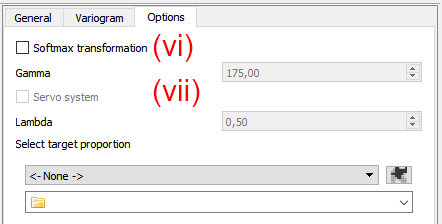
\includegraphics[width=0.5\textwidth]{modelagem_geologica/options_plugin}
	\end{center}
	%\legend{Fonte: Modificado de \citeonline{maureira}}
\end{figure}

Como \textit{output}, o \textit{plugin} gera, caso nenhuma opção da aba \textit{options} tenha sido selecionada, uma propriedade com o nome \textit{geo\_model}. Esse é o modelo geológico baseado na menor distância estimada para cada bloco. Ao marcar a opção \textit{softmax transformation}, uma propriedade \textit{Probability RTX} é criada, para cada litologia, onde $X$ é o algarismo que representa aquela litologia. Caso a opção \textit{servo system} seja selecionada, as propriedades \textit{Geologic\_Model\_Servo\_System} e \textit{Geologic\_Model\_Corrected} são criadas. A primeira representa o modelo criado a partir das probabilidades atualizadas e a segunda representa esse modelo suavizado (a correção é aplicada aqui uma única vez).

O quadro Algoritmo 2 abaixo mostra o funcionamento do algoritmo.

\begin{algorithm}[!ht]
\KwIn{Banco de dados categórico, propriedades \textit{signed distances RTX}, estratégia de krigagem, modelos variográficos, proporção alvo e parâmetros}
\KwOut{Propriedades \textit{geo\_model}, \textit{Probability RTX}, \textit{Geologic\_Model\_Servo\_System} e \textit{Geologic\_Model\_Corrected}}
\For{cada propriedade \textit{signed distances RTX}}{
Chama a krigagem ordinária no \textit{SGeMS} com os parâmetros imputados pelo usuário e interpola as distâncias calculadas para cada nó do grid informado\;}
\For{cada nó do grid}{Carimba no nó a categoria referente à menor distância estimada}
Cria a propriedade \textit{geo\_model}, baseada na menor distância interpolada\;
\If{opção \textit{softmax transformation} marcada}{
\For{cada propriedade interpolada}{
	\For{cada nó do grid}{Tranforma cada distância interpolada em probabilidade daquele nó pertencer a uma das litologias

}Cria uma propriedade \textit{Probability RTX} para cada litologia}
}
\If{opção \textit{servo system} marcada}{
Gera caminho aleatório\;
\For{nó do grid em caminho aleatório}{
Atualiza a proporção corrente marginal de cada categoria\;
\For{cada propriedade \textit{Probability RTX}}{
Atualiza as probabilidades de cada nó pertencer a cada uma das litologias de acordo com a diferença entre a proporção alvo e a proporção corrente marginal
}}
Cria a propriedade \textit{Geologic\_Model\_Servo\_System}\;
Suaviza o modelo e cria a propriedade \textit{Geologic\_Model\_Corrected}
}
Carimba nos blocos a categoria correspondente ao dado colocado
\caption{Interpolator}
\end{algorithm}

\section{Validação}

Os \textit{plugins} desenvolvidos foram validados tendo como referência resultados análogos da rotina \textit{DFMod} da biblioteca de algoritmos geoestatísticos \textit{GSLib}. Foi utilizado um banco de dados em três dimensões que possui 3276 amostras de 5 categorias diferentes para a validação do cálculo da função distância e modelo gerado a partir das distâncias estimadas. Ainda foi utilizado o \textit{jura data set} \cite{goovaerts1997geostatistics} para validação da \textit{softmax transformation} e \textit{servo system}.

Distâncias anisotrópicas foram calculadas com os parâmetros da \autoref{valid_rot}, escolhidos de forma arbitrária. E os resultados comparados.

\begin{table}[!ht]
\centering
\caption{Ângulos de rotação e proporções entre as direções principais usadas no cálculo da função distância anisotrópica.}
\label{valid_rot}
\begin{tabular}{lccc}

Rotações   & 30º & 45º & 60º \\ \hline
Proporções & 2  & 5  & 9  \\ 
\end{tabular}
\end{table}

A \autoref{dist_valid} mostra os \textit{scatterplots} entre as distâncias calculadas com o \textit{plugin} desenvolvido, no eixo $y$, contra as calculadas a partir da rotina \textit{DFMod} do \textit{GSLib} no eixo $x$, para todas as cinco categorias do banco de dados. A correlação é perfeita (100\%) para todos os gráficos.

\begin{figure}[H]
	\caption{\label{dist_valid}\textit{Scatterplot} entre as distâncias calculadas pelo \textit{plugin} desenvolvido contra distâncias calculadas a partir da rotina \textit{DFMod} do \textit{GSLib}.}
	\begin{center}
		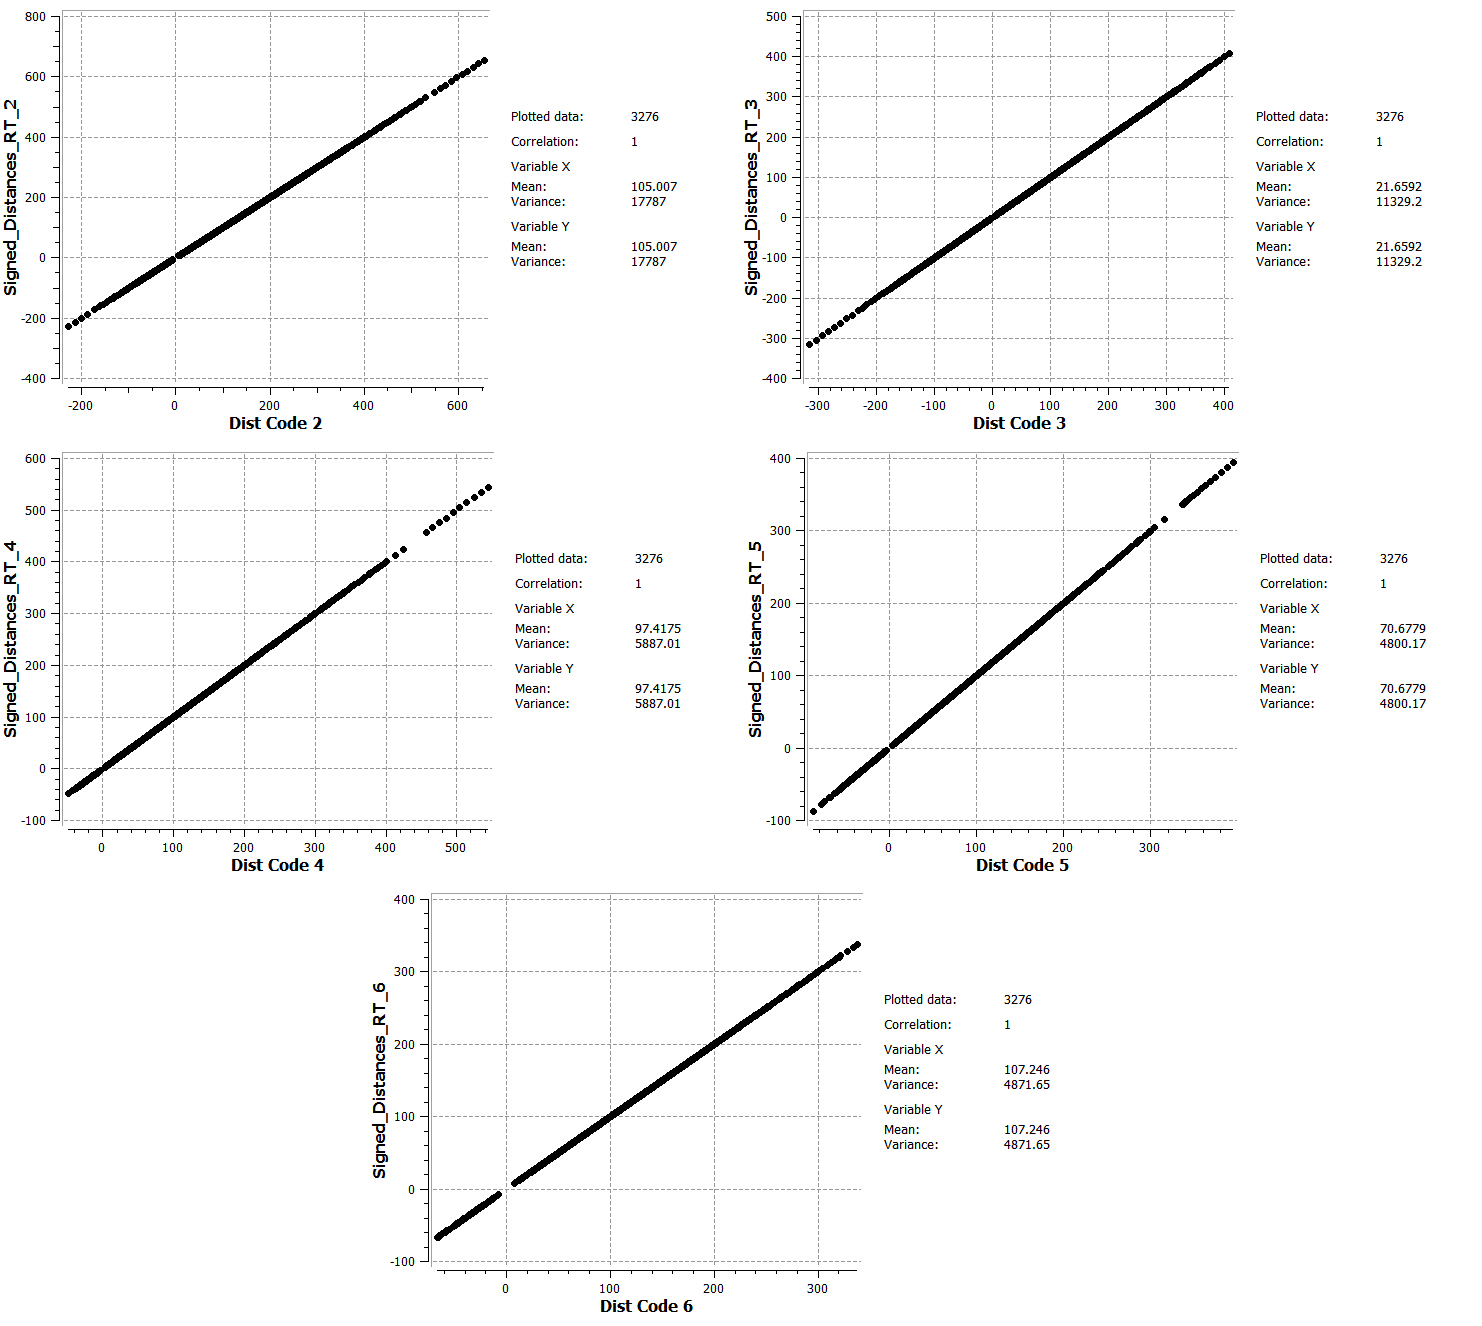
\includegraphics[width=0.8\textwidth]{modelagem_geologica/distances_valid}
	\end{center}
	%\legend{Fonte: Modificado de \citeonline{maureira}}
\end{figure}

Dois modelos foram gerados a partir dos  parâmetros do \autoref{anexo}. E foram comparados, novamente, em um \textit{scaterrplot} categórico (\autoref{model_valid}). O modelo gerado pelo \textit{plugin} desenvolvido aparece no eixo $y$, e no eixo $x$, o modelo criado a partir da rotina \textit{DFMod} do \textit{GSLib}. 99,998\% dos blocos são concordantes em ambos os modelos, blocos concordantes caem sobre a linha x=y e blocos discordantes fora dela, existem apenas três blocos discordantes entre os modelos gerados. 100\% de blocos concordantes não pôde ser atingido devido a diferença entre os códigos e linguagens de programação, as rotinas do \textit{GSLib} são escritas em \textit{fortran 90} enquanto o \textit{SGeMS} e seus \textit{plugins}, em \textit{C++} e \textit{python}, respectivamente.

\begin{figure}[H]
	\caption{\label{model_valid}\textit{Scatterplot} entre os modelos criados pelo \textit{plugin} desenvolvido e rotina \textit{DFMod} do \textit{GSLib}.}
	\begin{center}
		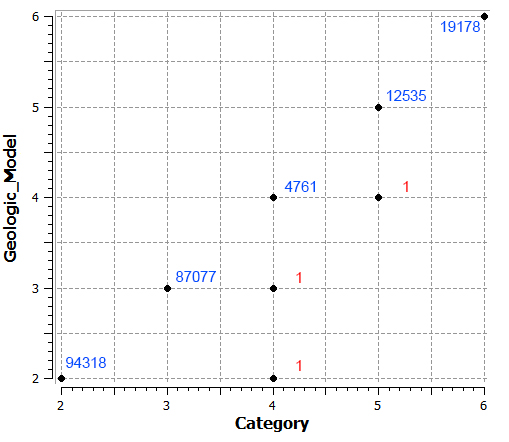
\includegraphics[width=0.8\textwidth]{modelagem_geologica/validation_models1}
	\end{center}
	%\legend{Fonte: Modificado de \citeonline{maureira}}
\end{figure}

Em nenhuma das versões do \textit{DFMod} encontradas nos repósitórios do \textit{GSLib} há versões funcionais, tanto da \textit{softmax transformation} quanto do \textit{servo system}. Então, como alternativa para validação, a correção \textit{servo system} foi executada no banco de dados jura, com um parâmetro $\lambda=0,99$. Dessa forma, é esperado que se, tanto o algoritmo da \textit{softmax transformation} quanto o algoritmo do \textit{servo system} (que depende do último), estejam corretos a proporção alvo seja reproduzida, ou pelo menos que um resultado bastante próximo seja obtido, já que não é possível usar um fator $\lambda=1$ (divisão por zero), que acarretaria na máxima correção possível, isto é, histogramas idênticos.

A \autoref{servo_valid} mostra os histogramas do modelo baseado somente nas distâncias estimadas à esquerda, dos dados ao centro (este foi utilizado como alvo para o \textit{servo system}), e do modelo após execução do \textit{servo system} à direita. As proporções alvo foram quase reproduzidas com perfeição, a diferença entre as médias dos histogramas é menor que 0,01.

\begin{figure}[H]
	\caption{\label{servo_valid}Histogramas do modelo baseado somente nas distâncias estimadas à esquerda, dos dados ao centro, e do modelo após execução do \textit{servo system} à direita.}
	\begin{center}
		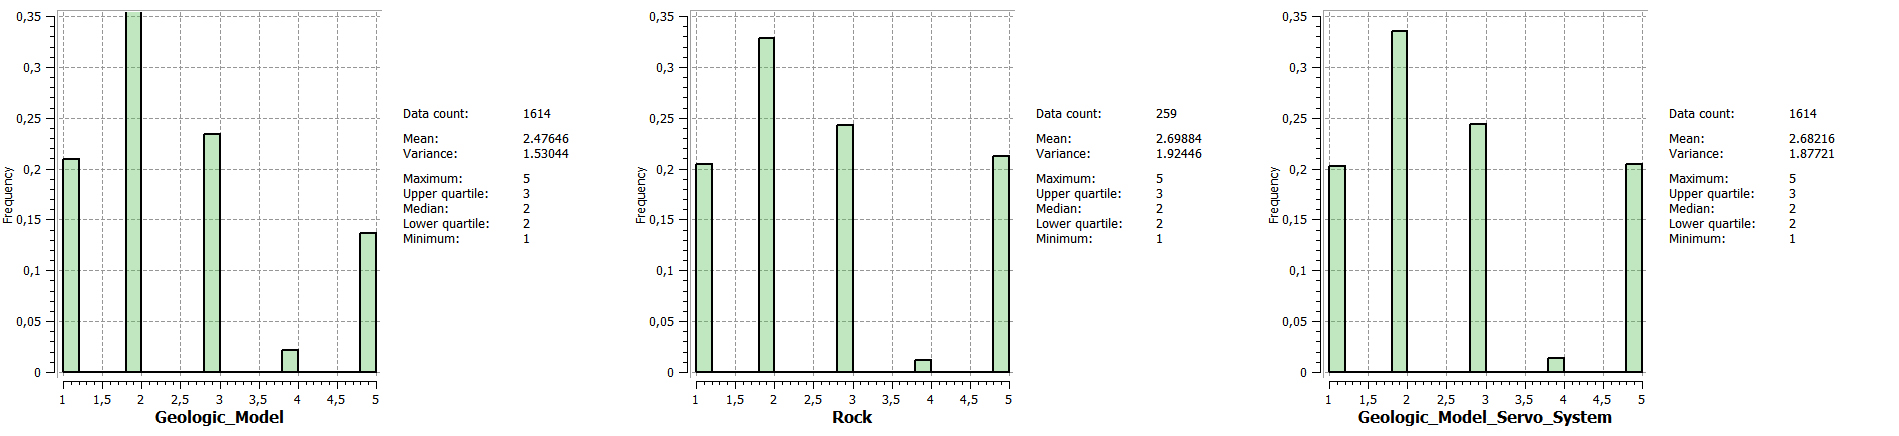
\includegraphics[width=\textwidth]{modelagem_geologica/servo_valid}
	\end{center}
	%\legend{Fonte: Modificado de \citeonline{maureira}}
\end{figure}